In the previous chapter, we have learned how compilation to high-level targets can present an easy way of implementing a compiler.
These compilers generated outputs which were still platform independent and portable.
However, compilers can also target a specific computer architecture directly, thus removing another layer of abstraction.
The concept of compiling to a specific architecture directly is similar to the VM since its compiler also targets its architecture directly.
However, implementing a compiler targeting the architectures presented in this chapter has proven to be a lot more demanding since the VM uses a fictional architecture purposefully developed for this paper.
Reasons for this chapter's difficulty mostly include target-specific constraints which were
still irrelevant in the previous chapter.
This chapter contains the term \enquote{low-level} in its name since the presented compilers
generate code for specific target-architectures directly.

\section{Low-Level Programming Concepts}
Programming using high-level languages does not require knowledge about the target architecture of the program.
However, in this chapter, two compilers targeting the low-level assembly language are presented.
In order to make sections in which these compilers are explained more approachable,
some of the most important low-level programming concepts are explained in this section.
We will only explain concepts which play a significant role later on.

\subsection{Sections of an ELF File}
Since a program needs to be representable in a low-level manner, special formats are often required.
ELF stands for \enquote{executable and linkable format} and is often found on unix-like systems like Linux.
Programs using the ELF format can be represented in three different types of files.
For instance, object files generated by a compiler, like in the previous LLVM section, might use the ELF format.
Furthermore, libraries using \emph{shared object files} might also leverage the ELF format.
Most executable program use the format in order to represent a structured container for instructions, data, and additional information.
This way, the unit is mostly self-contained and can be executed by the operating system easily.
Therefore, ELF describes the format of a class of files and not just of an individual type of file~\cite[p.~74-76]{Zhirkov2017-wk}.

Even though a processor only has access to one physical memory unit for both instructions and program data,
most assembly programs like to separate these types of memory into their separate components.
Therefore, an object file and assembly program is divided into so-called \emph{sections}~\cite[p.~19]{Zhirkov2017-wk}.
% Object files using the ELF format are usually partitioned into several sections.
% Here, every individual section exists to serve a special purpose.
% For instance, the \qVerb{.text} section stores all CPU instructions to be executed.
% Furthermore, the \qVerb{.data} and \qVerb{.rodata} sections store mutable and read-only data respectively~\cite[p.~76]{Zhirkov2017-wk}.
In ELF programs, some of the important sections are:
\begin{itemize}
	\item \texttt{.text} stores the logic of the program represented using CPU instructions
	\item \texttt{.rodata} stores read-only global data, it is often used for global constants.
	\item \texttt{.data} stores mutable global data, such as mutable global variables
\end{itemize}

Even though a typical ELF file also contains other sections,
this list only includes entries which are of importance later in later sections of the paper~\cite[p.~76]{Zhirkov2017-wk}.

\subsection{Assemblers and Assembly Language}

\begin{wrapfigure}{R}{.27\textwidth}
	\centering
	\begin{tikzpicture}[node distance=1cm, inner sep=3mm]
		\node (lexical_analysis) [entity, fill=none] {High-level languages\\(\emph{C}, \emph{Rust}, \emph{rush})};
		\node (syntactic_analysis) [entity, below=of lexical_analysis, align=center] {Assembly language\\level};
		\draw [arrow] (lexical_analysis) -- (syntactic_analysis);
		\node (semantic_analysis) [entity, fill=none, below=of syntactic_analysis, align=center] {Machine language\\level};
		\draw [arrow] (syntactic_analysis) -- (semantic_analysis);
		\node (codegen) [entity, fill=none, below=of semantic_analysis] {Operating system \\ and Hardware level};
		\draw [arrow] (semantic_analysis) -- (codegen);
	\end{tikzpicture}
	\caption{Level of Abstraction provided by Assembly}\label{fig:abstractions}
\end{wrapfigure}

Assembly language describes a type of low-level programming languages which are directly influenced by the target architecture.
Since the assembly code provides a slight abstraction over the computer's hardware,
the assembly code must be translated to machine code before it can be executed.
This process is performed by a program named the \emph{assembler} and is often called \emph{assembly}.
A typical characteristic of assembly code is that it seems relatively cryptic to a human reading it.
Furthermore, compared to high-level languages like C, assembly code is relatively low-level since it can be used to interact with the hardware directly.

For instance, the RISC-V instruction \qVerb{add a0, a0, 2} would be used in integer addition.
This example contains most characteristics of an assembly language program.
Like hinted previously, the name of the instruction is a mnemonic.
In this case, \qVerb{addi} stands for \enquote{add immediate}.
Furthermore, the exact semantic meaning of the instruction is not immediately apparent.
At last, the instruction for adding integers differs for most CPU architectures.
For instance, an equivalent instruction for the x\_86 architecture could be `\texttt{add \%rdi, 2}'.
Therefore, the fact that instructions differ on each target architecture is clearly apparent.

As seen above, the application code in form of instructions is placed in the \qVerb{.text} section of an ELF binary.
In most assembly dialects, the programmer is able to partition the code manually using sections.
If the assembly code is assembled to an ELF object file, the \qVerb{.text} section of the assembly should contain all the instructions.
Just like parts of the LLVM IR, the \qVerb{.text} section of an assembly program obeys a hierarchy.
This section contains many labels which mark the beginning of a new basic block.
However, these basic blocks do not come with all the constraints which are to be followed when using LLVM IR\@.
For instance, a block in assembly might even contain no instructions, does not have to be terminated and could even be terminated twice.
Here, terminating instructions mean jump- and return-instructions.
Therefore, the constraints in assembly are much weaker than the ones introduced by LLVM\@.
Because an assembly usually omits complex optimizations, struct rules constraining the assembly code can be omitted too.

Since assembly provides significantly less abstraction than high-level languages, the question of how much abstraction is lost emerges.
In order to understand how much abstraction is provided by assembly, we should consider Figure~\ref{fig:abstractions}.
Here, the highest level of abstraction is provided by high-level programming languages like C or Rust.
In the context of this paper, rush presents roughly the same level of abstraction like these languages.
The next lower level of abstraction is provided by assembly.
Now, the program is no longer independent of its target architecture and is much more demanding to furmulate.
However, the next lower level of abstraction below assembly is represented by code in machine language.
As of today, one only rarely encounters a programmer writing programs using this level of abstraction.
Since the machine language program is represented in binary, it is nearly impossible for a human to write or understand.
However, the machine language is also just an abstraction of the computer's hardware and operating system.
Therefore, assembly provides enough abstraction to be comprehensible for a human whilst being a low-level representation of the program.
Although assembly provides more abstraction than the two levels at the bottom of the figure, programmers rarely program in assembly directly.
Some benefits of using assembly language to formulate a program are increased runtime efficiency and decreased code size whilst having fine-grained control over the hardware and operating system.
Therefore, it might be reasonable for a compiler to generate assembly code from the source program.
This way, the program is translated into a low-level, target-specific representation which allows the program to be executed on the target machine directly.
However, an assembler is still required in order to translate the assembly output of the compiler.
Since most assemblers output object files, a linker is required to create the final executable program.
Therefore, a compiler targeting the assembly of a specific architecture depends on these two additional steps before the program can be executed~\cite[p.~5-6]{Dandamudi2005}.

One might argue that the compiler could output object files directly.
However, doing so rarely creates any significant benefits other than the omitted dependence on the assembler.
Furthermore, implementing a compiler using this approach often significantly increases the complexity of the compiler since it now has to perform the role of the assembler as well.
However, the compiler could also emit binary data directly, thus making its implementation significantly more demanding.

\subsection{Registers}

\begin{wrapfigure}{R}{0.5\textwidth}
	\centering
	\begin{tikzpicture}[node distance=2cm]
		\node(CPU)[center] {CPU};
		\node(registers)[entity, left of=CPU, yshift=3cm, vstack=4, rectangle split part align=left] {
			Registers
			\nodepart{two}{\texttt{r0}}
			\nodepart{three}{\texttt{r1}}
			\nodepart{four}{\ldots}
		};
		\node(memory)[entity, right of=CPU, yshift=3cm] {Memory};

		% TODO: Maybe use `arrow` instead of `relation` in order to remove spacing
		\draw [darrow, very thick, double] (CPU) -- node[anchor=east, yshift=-.1cm] {fast} (registers);
		\draw [darrow] (CPU) -- node[anchor=west] {slow} (memory);
	\end{tikzpicture}
	\caption{Relationship Between Registers, Memory, and the CPU}\label{fig:cpu_reg_mem}
\end{wrapfigure}

Most processors contain numerous registers in order to hold data, instructions, and state information.
In a computer, registers are sometimes used to hold data stored in variables.
However, most of the time, registers are used as temporary storage in large computations.
Registers are used in the latter case because they are way faster than memory.
Therefore, an algorithm using registers instead of memory will usually run faster.
However, even though registers are faster than memory, they are not used all the time.
This is because CPU registers are a limited resource, meaning every register-based CPU only has a finite amount of registers available.
Registers should therefore be used carefully and only when they are really needed~\cite[pp.~212-214]{Watson2017}.

Figure~\ref{fig:cpu_reg_mem} shows how the CPU interacts with its registers and the computer's memory.
The connection between the set of registers and the CPU is marked as a short and thick arrow because the connection between the CPU and its registers is very short and fast.
Although the registers are often physically parts of the CPU, they are displayed as separate entities in this example.
For the memory, the arrow is long and thin.
This represents the long and therefore slow connection between the CPU and the memory modules.
In most modern computers, this connection often spans across several centimeters on the motherboard.
Therefore, higher latency during memory access is inevitable~\cite[pp.~20-21]{Dandamudi2005}.

Nearly every CPU architecture will include an individual register layout, differing in size, count, and type.
Therefore, the exact information about registers always depends on which CPU is used.
As a rule of thumb, having more registers in an architecture will almost always improve performance of that architecture.
Furthermore, not every register is identical.
There might be platforms with some general-purpose, some floating-point, and some special-purpose registers.
For instance, there may be registers which contain information about the CPU's current instruction.
Furthermore, common architectures also include special-purpose registers for modifying the machine's memory.
Therefore, there is nearly always an appropriate register matching the requirement~\cite[Chapter~2]{Dandamudi2005}.

\Lirsting[wrap=L, raw=true, ranges={4-6}, wrap width=0.3\textwidth, caption={Example Assembly Program for Explaining Register Allocation}, label={lst:register_alloc}]{listings/register_alloc_simple.s}

For a compiler, the limited amount of registers presents a big challenge.
Some architectures may require that the operands of arithmetic or logical instructions have been explicitly loaded into registers beforehand.
In this case, registers would be required in nearly all computations.
In order to understand how registers management can present a challenge, Listing~\ref{lst:register_alloc} should be considered.
This snippet displays RISC-V assembly instructions which calculate the sum of the two integers 40 and 2.
In line 4, the integer value 40 is placed in the register \qVerb{a0}.
In line 5, another integer, this time 2 is placed in \qVerb{a1}.

Next, the \qVerb{add} instruction is used to calculate the sum of these two integers.
Since the first operand of the instruction specifies the register in which the result should be placed,
the original value of 40 in the register \qVerb{a0} would be overwritten by the instruction~\cite[reference]{Patterson2017}.
Through this example, it becomes apparent that other instructions might use registers unexpectedly.
Therefore, subtle bugs can be created if an instruction overwrites registers.

In compilers, the process of \emph{register allocation} is responsible for managing how registers are used.
This process attempts to use registers in a way leading to maximized efficiency of the output program.
Since accessing registers is often faster, a register allocator will try to use registers as often as possible.
Production-ready compilers often try to keep as much of the frequently accessed data in registers.
For instance, this frequently accessed data may also include variables which are normally saved in memory.
It is apparent that in most programs, the number of variables will certainly exceed the capacity provided by registers.
Therefore, register allocation has to detect when no free registers are available anymore.
In this case, the compiler has to save data in memory instead of registers.
This process of saving excess data in memory instead of registers is called \emph{register spilling}.
Since register spilling introduces a performance penalty, register allocation algorithms often attempt to prevent it as much as possible.
Therefore, sophisticated algorithms for register allocation are often mandatory as long as the factor of output code performance is non-trivial.

Apart from just managing the use of registers, most allocation algorithms are responsible for many other register-related tasks.
For instance, register allocation should detect when a variable is no longer needed so that its register can be freed.
Moreover, register allocation has to ensure that no conflicts between registers are introduced.
Such a conflict may be that a register is accidentally overwritten by an instruction in a completely unrelated basic block.
It is apparent that an algorithm performing all these tasks can not be implemented in an ad-hoc manner.
Instead, this process often requires complex graph algorithms for determining which registers can be used and freed.
Therefore, implementing register allocation in a compiler is often a very demanding task~\cite[pp.212-214]{Watson2017}.
Since register allocation represents a complex topic, it will not be explained any further.

\subsection{Using Memory: The Stack and the Heap}
\TODO{@RubixDev: write this subsection}\\
\TODO{Useful information:~\cite[p.~99]{Patterson2017-zq}}\\
\TODO{Insert figure which uses \qVerb{drawstack.sty}}

\begin{itemize}
	\item Repetition: When is the stack used instead of registers?
	\item Insert very figure of the stack.
    \item Only mention that there are stack pointers and why they are needed; do not explain how they point / behave exactly
    \item Stack can be indexed
\end{itemize}

\subsection{Calling Conventions}

Programmers often use \emph{procedures} or \emph{functions} in order to structure their programs,
both to make the program easier to understand and to allow shared logic to be reused.
Therefore, procedures allow the programmer to focus on one portion of the tasks at the time.
Often, parameters and returned values act as the interface between the procedure and the remaining code.
Therefore, procedures present one way of how a high-level programming language might provide abstraction.
During a procedure call in a high-level language like rush, many individual steps need to be performed in the program's low-level representation.
Since assembly does not support the use of high-level functions, most architectures specify their own \emph{calling convention} which describes how low-level function calls are to be performed.
On most architectures, a low-level procedure call might take place like the following steps:

\begin{itemize}
	\item The caller places the call arguments in a place where the procedure can access them.
	\item Control is transferred to the procedure, often using a jump or specialized call instruction.
        This specialized instruction often saves the \emph{return address}\footnote{A link to the caller site, allows the called procedure to jump back to the caller~\cite[p.~99]{Patterson2017-zq}.} in a special register so that function returns are easier.
	\item The first task the called function performs is acquiring local storage resources needed by the procedure.
	      Often, registers are spilled if required.
	      Furthermore, stack memory for the procedure's local variables is often allocated in this step.
	\item Internal code of the procedure is run by executing the function body's instructions.
	\item The procedure's result value is placed somewhere so that the caller can access it.
	      Here resources allocated in step 3 are also released again.
	\item Control is transferred back to the caller using a specialized return-instruction.
	      A specialized instruction is often required since procedures can be called from multiple places in the program.
	      Therefore, the return-instruction jumps back to the instruction which had initiated the function call.
\end{itemize}

In order to leverage optimal performance during function calls, passed arguments are usually kept in registers.
However, in the previous subsection about registers, we have learned that most architectures state that only subset of their registers are to be used as function arguments.
Therefore, if a function is called using more than eight arguments, every remaining argument has to be spilled to memory.
In this case, each additional parameter of the function is placed inside the stack frame of the called function so that it can access it.~\cite[p.~98]{Patterson2017-zq}.

For instance, a target architecture might provide \emph{four} registers which can hold function arguments.
Now, a function is called using \emph{six} arguments.
Here, register spilling is mandatory since there are two more arguments than registers.
Figure~\ref{fig:call_conv_spill} illustrates how such a call would be managed on this fictional architecture.

\begin{wrapfigure}{L}{0.3\textwidth}
	\centering
	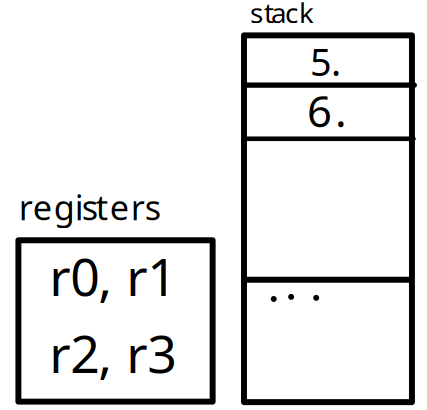
\includegraphics[width=.2\textwidth]{./calling_convention_draft.png}
	\caption{\textcolor{red}{DRAFT:} Spilling Registers for Function Calls}\label{fig:call_conv_spill}
\end{wrapfigure}

Here, the registers \qVerb{r0} — \qVerb{r3} contain the first four argument values.
The excess arguments which could not fit into registers are now placed on the stack.
Even though argument 5 and 6 are placed on top of the stack in this example,
the exact location of spilled call arguments differs for every architecture.

For managing the calling convention in assembly, most functions contain a \emph{prologue} and an \emph{epilogue}.
These blocks of the function are responsible for allocating and deallocating resources which the function might use.
For instance, the stack- and frame-pointer is often adjusted in the prologue.
This way, space on the stack is allocated for variable declarations found in the called function.
However, the modification offset always depends on how much memory the called function will require during runtime.
Therefore, a compiler would have to keep track of the count of variable declarations made by a function.
Apart from allocating stack space, the prologue is also often used for storing special registers on the stack.

The epilogue however is required for deallocating all resources which were previously allocated by the function's prologue.
For instance, the stack-related pointers are modified to reflect their state before the function call.
Furthermore, any special registers previously saved on the stack are now restored.
Obviously, a return-statement should always jump to the function's epilogue instead of terminating the function directly.
At the end of most epilogues, a return-instruction jumping back to the caller location is often found.
Therefore, the prologue is executed as the first code when calling the function and the epilogue is called as the last code before this function terminates.

It is to be mentioned that implementing a compiler which respects the calling convention of its target architecture is not required.
However, following the convention is often reasonable in order to preserve \emph{ABI}\footnote{Short for \enquote{application binary interface}, allows calling foreign functions from another program} compatibility of the compiled program.
